\documentclass[a4paper,12pt]{report}
\usepackage[utf8]{vietnam}
\usepackage{graphicx}
\usepackage{fancybox}
\usepackage{longtable}
\usepackage{listings}
\usepackage{relsize}
\usepackage{cases} 
\usepackage[left=3cm, right=2.00cm, top=2.00cm, bottom=2.00cm]{geometry}
\lstset{
   %keywords={break,case,catch,continue,else,elseif,end,for,function,
   %   global,if,otherwise,persistent,return,switch,try,while},
   basicstyle=\ttfamily \fontsize{12}{15}\selectfont,   
	% numbers=left,
   frame=lrtb,
tabsize=2
}
\setlength{\parskip}{0.6em}
\usepackage{hyperref}
\usepackage{float}
\hypersetup{
    colorlinks,
    citecolor=black,
    filecolor=black,
    linkcolor=black,
    urlcolor=black
}
\usepackage[nottoc]{tocbibind}
\usepackage[english]{babel}
\usepackage{indentfirst}
\addto\captionsenglish{%
 \renewcommand\chaptername{Phần}
 \renewcommand{\contentsname}{Mục lục} 
 \renewcommand{\listtablename}{Danh sách bảng}
 \renewcommand{\listfigurename}{Danh sách hình vẽ}
 \renewcommand{\tablename}{Bảng}
 \renewcommand{\figurename}{Hình}
 \renewcommand{\bibname}{Tài liệu tham khảo}
}
\begin{document}
\thispagestyle{empty}
\thisfancypage{
\setlength{\fboxrule}{1pt}
\doublebox}{}
\begin{center}
{\fontsize{16}{19}\fontfamily{cmr}\selectfont TRƯỜNG ĐẠI HỌC BÁCH KHOA HÀ NỘI\\
VIỆN CÔNG NGHỆ THÔNG TIN VÀ TRUYỀN THÔNG}\\
\textbf{------------*******---------------}\\[1cm]

\includegraphics[scale=0.13]{hust.jpg}\\[1.3cm]

{\fontsize{32}{43}\fontfamily{cmr}\selectfont BÁO CÁO}\\[0.1cm]
{\fontsize{38}{45}\fontfamily{cmr}\fontseries{b}\selectfont MÔN HỌC}\\[0.2cm]
{\fontsize{19}{20}\fontfamily{phv}\selectfont Tính toán khoa học }\\[0.2cm]
{\fontsize{13}{20}\fontfamily{cmr}\selectfont Đề tài: Mạng Google Inception trong bài toán phân loại}\\[2.5cm]
\end{center}
\hspace{1cm}\fontsize{14}{16}\fontfamily{cmr}\selectfont \textbf{Nhóm sinh viên thực hiện:}

\begin{longtable}{l c c}

Họ và tên & MSSV  & Lớp\\
Nguyễn Tuấn Đạt & 20130856 & CNTT2.02-K58 \\
Đặng Quang Trung & 20134145 & CNTT2.02-K58 \\
Phan Anh Tú & 20134501 & CNTT2.01-K58 \\
\end{longtable}

\hspace{0.6cm}\fontsize{14}{16}\fontfamily{cmr}\selectfont \textbf{Giảng viên môn học: }TS. Đinh Viết Sang \\[1.5cm]
\begin{center}
\fontsize{16}{19}\fontfamily{cmr}\selectfont Hà Nội 1--2017

\end{center}
\newpage

\pdfbookmark{\contentsname}{toc}
\tableofcontents
\listoffigures


\phantomsection
\addcontentsline{toc}{chapter}{Lời cảm ơn}
\chapter*{Lời cảm ơn}
Chúng em xin chân thành cảm ơn Thầy giáo, TS. Đinh Viết Sang đã tận tình giảng dạy, hướng dẫn chúng em thực hiện đề tài này. Trong quá trình thực hiện, đề tài của chúng em không tránh khỏi những hạn chế, thiếu sót, chúng em rất mong nhận được những ý kiến đánh giá, nhận xét của Thầy để đề tài này có thể được hoàn thiện hơn.


\chapter{Đặt vấn đề}
Trong bối cảnh nghành công nghiệp công nghệ thông tin đang phát triển rất mạnh mẽ ngày này, có lẽ Deep Learning là một trong những từ khóa được quan tâm nhất. Deep Learning đang được ứng dụng ngày càng rộng rãi trong các công việc của cuộc sống hàng ngày như: ô tô tự lái, nhận diện giọng nói, nhận diện khuôn mặt ....
\par Là một sinh viên ngành khoa học máy tính, chúng em nhận thấy cần trang bị những kiến thức cần thiết về Deep Learning. Vì vậy, mục tiêu của bài tập lớn này của chúng em là tìm hiểu về Deep Learning và cụ thể là tìm hiểu về mạng Google Inception trong bài toán phân loại.
\par Google Inception hay  GoogleNet là mạng biến thể của mạng Convolutional neural network (A deep convolutional neural network architecture \cite{googlenet}). Convolutional neural network (CNN) là một dạng của mạng neuron nhân tạo thông thường (Artificial neural network - ANN) (những mạng này sẽ được chúng em giới thiệu ở phần sau của báo cáo).  
\par Phần tiếp theo của báo cáo bao gồm các phần sau: phần 1 và phần 2 giới thiệu về mạng ANN, CNN; các phần tiếp theo sẽ trình bày về mạng Google Inception và các cải tiến của nó. Cụ thể:
\par \textbf{Phần 1}
\par \textbf{Phần 2} 

\chapter{Giới thiệu học sâu}
\section{Mạng neuron nhận tạo}
Mạng neuron nhân tạo là một mô hình tính toán mô phỏng các hệ thống neuron sinh học. Mạng neron mà một cấu trúc được tạo nên bởi một số lượng các neuron liên kết với nhau.\\

Mỗi neuron thực hiện một tính toán cục bộ nhận đầu vào và đưa ra đầu ra tương ứng. Giá trị đầu ra của một neuron được xác định bởi : đặc tính vào ra, các liên kết của nó với neuron khác, có thể còn có các đầu vào bổ sung.

Chức năng của một  mạng neuron được xác định bởi :
\begin{itemize}
\item Kiến trúc
\item Đặc tính vào ra
\item Chiến lược học
\item Dữ liệu học 
\end{itemize}

Mạng neuron có khả năng học, nhớ lại, và khái quát hóa từ các dữ liệu học, bằng cách gán và điểu chỉnh các trọng số của các liên kết giữa các neuron.
\section{Học sâu}
Học sâu là một nhánh của học máy cơ sở trên một tập các thuật toán nhằm cố gắng mô hình hóa trừu tượng mức cáo trong dữ liệu bởi việc sử dụng với nhiều tầng xử lý. 

\begin{figure}[H]
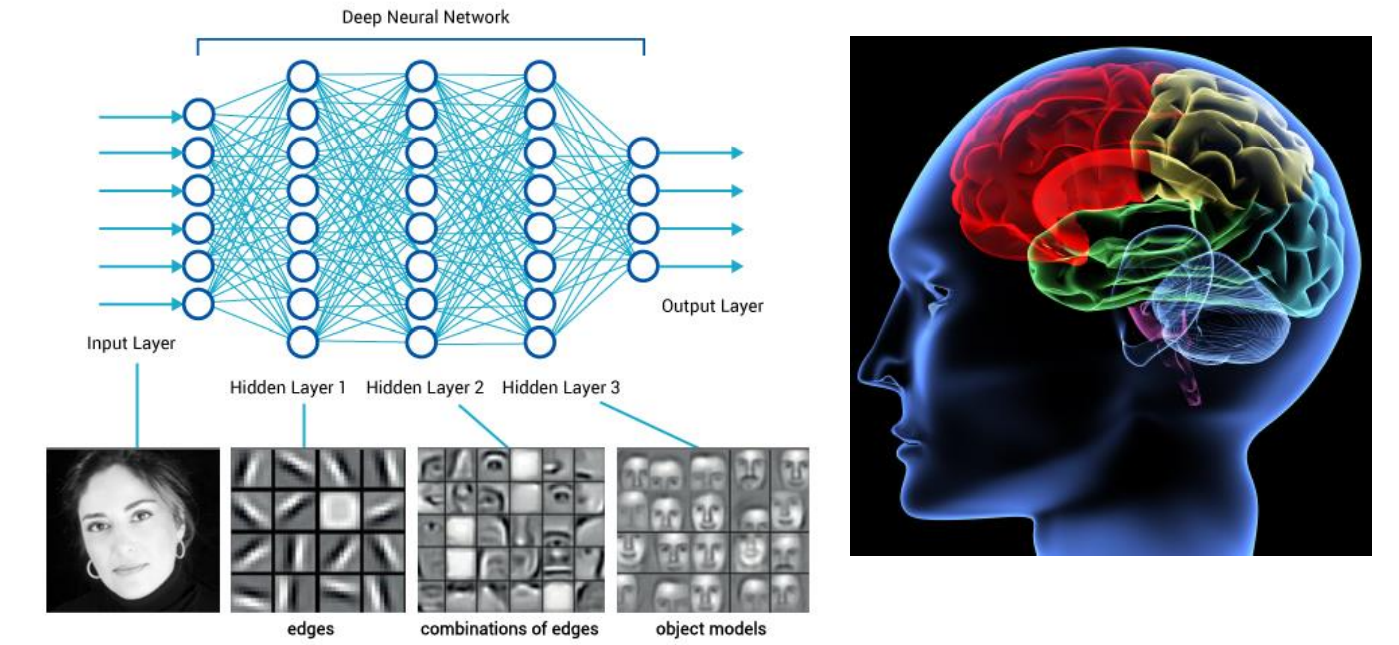
\includegraphics[scale=0.45]{deeplearning.png}
\caption{Mô tả mô hình một mạng neuron học sâu}

Một ví dụ cụ thể nhất về học sâu đó là một mạng neuron nhiều tầng (MLP). Nếu ta coi mạng MLP là một hàm thì hàm đó là hàm hợp của rất nhiều các hàm đơn giản khác.
\end{figure}

Lịch sử xu hướng của học sâu:
\begin{itemize}
\item Học sâu xuất hiện từ xưa nhưng đã dẫn không còn phổ biến do nhiều lí do
\item Học sâu đã trở lại  và trở nên rất hữu khi có rất nhiều dữ liệu để huấn luyện.
\item Mô hình học sâu phát triển nhanh chóng theo thời gian khi cơ sở hạ tâng cho học sâu ngày càng được cải thiện. 
\item Các vấn đề học sâu giải quyết được có độ phức tạp ngày càng tăng đi đôi với độ chính xác cũng vậy.
\end{itemize}
\section{Các thành phần quan trọng trong mô hình học sâu}
\begin{itemize}
\item Hàm mục tiêu:\\ Các hàm mục tiêu hay được sử dụng \begin{itemize}
\item sigmoid
\item tanh
\item ReLU
\item Maxout
\item ELU
\end{itemize}
\item Chiến lược học: \begin{itemize}
\item Stochastic Gradient Descent
\item Mini-batch Gradient Descent
\item SGD-Momentum
\item SGD-Vanilla
\item Adagrad
\item AdaDelta
\end{itemize}
\item Kiến trúc mạng
\item Thuật toán học: Hiện tại thuật toán lan truyền ngược vẫn là thuật toán được sử dụng rộng rãi và đem lại hiệu quả cao.
\end{itemize}

\chapter{Giới thiệu mạng CNN}

\chapter{GoogleNet}
Trong phần này chúng em sẽ trình bày về kiến trúc của mạng Google Inception (GoogleNet), nhưng trước hết trong phần đầu tiên chúng em sẽ giới thiệu tổng quan về mạng GoogleNet, mục đích khi thiết kế mạng, những ưu điểm của nó so với các mạng khác trong bài toán phân loại.

\section{Tổng quan về GoogleNet}
Inception là một biến thể của mạng CNN (a deep convolutional neural network architecture \cite{googlenet}), một trong những khác biệt lớn nhất của kiến trúc này là sự cải thiện của tài nguyên tính toán bên trong mạng (mặc dù mạng tăng cả về chiều sâu (số lượng tầng trong mạng) và chiều rộng (số lượng neural trong một tầng) nhưng chi phí tính toán vẫn không đổi (chi phí để học các trọng số trong mạng)) (Mạng GoogleNet trong ILSVRC 2014 (ImageNet Large-Scale Visual Recognition Challenge) có số lượng tham số ít hơn 12 lần với kiến trúc mạng đã chiến thắng năm 2012). 


\section{Inception Module}	



\begin{thebibliography}{9}
\bibitem{googlenet} C. Szegedy, W. Liu, Y. Jia, P. Sermanet, S. Reed, D. Anguelov, D. Erhan, V. Vanhoucke, and A. Rabinovich. \textit{Going deeper with convolutions}

\bibitem{rethinking} C. Szegedy, V. Vanhoucke, S. Ioffe, J. Shlens, and Z. Wojna. \textit{Rethinking the inception architecture for computer vision}

\bibitem{inceptionv4} C. Szegedy, S. Ioffe, and V. Vanhoucke. \textit{Inception-v4, Inception-ResNet and the Impact of Residual Connections on Learning}

\end{thebibliography}

\end{document}
